\chapter{Modelos de comportamiento}
\label{ch:sota-behavior-models}

El objetivo que perigue la simulación de tráfico es hacer cada vez más realistas los modelos generados. En un modelo basado en \gls{mas}\sidenote{Donde cada uno de los agentes trabaja de manera independiente sobre el mismo problema, esto es, el tráfico.}, el realismo aumenta cuanto más se asemeja el comportamiento de un agente al de un conductor real.

¿A qué nos referimos cuando hablamos del "comportamiento"? Según el diccionario de la real academia, \enquote{comportar} se define como \textit{actuar de una manera determinada}. Sin embargo, no queda claro qué factores constituyen el comportamiento al volante, es decir.

Conducir implica la ejecución de múltiples tareas en paralelo, cada una de diferente nivel cognitivo. Además, las acciones no está limitadas a la interacción con el vehículo; el conductor ha de tener en cuenta otros factores como, por ejemplo, la situación de tráfico en la que se encuentra inmerso, las señales, los peatones o los dispositivos \gls{its}.

\begin{figure}
	\centering
	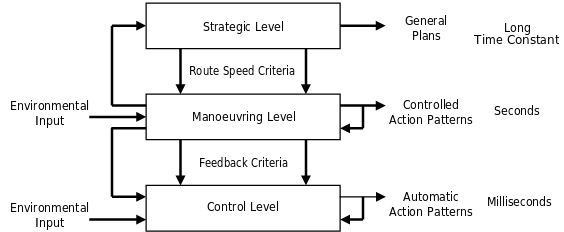
\includegraphics{three-levels-of-human-driving}
	\caption{Los tres niveles jerárquicos que describen la tarea de conducción según~\cite{michon1985critical}: \textit{estrategia} (i.e. las decisiones generales), la \textit{maniobra} (i.e. decisiones durante la conducción de más corto plazo) y \textit{control} (i.e. comportamientos automáticos). (\TODO{Rehacer la figura nosotros, esta no me gusta. Es del \cite{michon1985critical}}).}
	\label{fig:three-levels-of-human-driving}
\end{figure}

Michon en \cite{michon1985critical} divide en tres los niveles de abstracción de las tareas: el de \textbf{control}, que se ocupa de las tareas de más bajo nivel destinadas éstas a mantener la conducción como son la aceleración o los cambios de marcha, el de \textbf{maniobra} o táctico, donde sus tareas son las encargadas de mantener la interacción con el entorno como los cambios de carril o el control de las señales y demás estímulos externos, y el \textbf{estratégico}, que engloba las tareas de más alto nivel como el razonamiento y la planificación de rutas (ver figura~\ref{fig:three-levels-of-human-driving}).

El comportamiento de un conductor al volante tiene una relación directa con el nivel de abstracción de maniobra o táctico. Ésta se puede concebir como la encargada de planificar acciones a corto plazo para conseguir objetivos a corto plazo. Las tareas de control son automáticas, y influyen poco o nada en las tomas de decisión relacionadas con tareas como cuánto acelerar en esta situación y cuándo cambiar de tráfico. Las tareas estratégicas estan a un nivel más alto de abstracción (e.g. la ruta a seguir hasta mi destino) y tampoco afectan demiasiado al comportamiento en situaciones concretas\sidenote{No obstante algunos autores (e.g. \TODO{Observation-based lane-vehicle-asignment hierarchy for microscopic simulation on an urban street network} o \cite{Toledo2003}) han demostrado que en ocasiones, la planificación de la ruta sí afecta a la preferencia de un conductor por un carril determinado.}.

En este capítulo se explorará qué modelos de interés dentro de la \gls{ci} se han desarrollado hasta el momento y cuáles son sus limitaciones.

\section{Tipos de maniobra}

En el nivel táctico del comportamiento, las tareas que se realizan durante la conducción son las relacionadas a circular con el vehículo dentro del flujo de tráfico, sin bajar demasiado de detalle. En la literatura, estas tareas se centran en dos clases diferentes (figura \ref{fig:behavior-model-classification}): las de \textbf{aceleración}, encargadas de modelar el comportamiento de un conductor en el carril en el que se encuentra y las de \textbf{cambio de carril}, encargadas de decidir y ejecutar los cambios de carril.

\begin{figure}
	\centering
	\begin{tikzpicture}
	\tikzset{every concept/.style={minimum size=2cm, text width=2cm}}
	\path[mindmap,concept color=MidnightBlue, text=white]
	node[concept] {modelos} [clockwise from=300]
	child[level distance=100, concept color=RoyalBlue] {
		node[concept] {aceleración} [clockwise from=30]
		child[concept color=Peach] {
			node[concept] {free-flow}
		}
		child[concept color=Peach] {
			node[concept] {car-following}
		}
	}
	child[level distance=100, concept color=RoyalBlue] {
		node[concept] {lane-changing} [clockwise from=210]
		child[concept color=Peach] {
			node[concept] {lane-selection}
		}
		child[concept color=Peach] {
			node[concept] {gap-acceptance}
		}
	};
	\end{tikzpicture}
	\caption{Las diferentes tareas para modelar el comportamiento de un conductor al volante. Están clasificadas en dos tipos, de aceleración, encargadas de definir cómo acelera el conductor en casos con y sin vehículo delantero y de lane-changing, encargadas de las tareas relacionadas con el cambio de carril.}
	\label{fig:behavior-model-classification}
\end{figure}

\subsection{Modelos de aceleración}

Se ocupan de gestionar el comportamiento del conductor sobre la aceleración (positiva o negativa) en un entorno lineal como lo es un carril de tráfico.

Se identifican dos comportamientos diferenciados dentro de este: el \textbf{\index{free-flow}} o circulación sin impedimento, donde el comportamiento del conductor viene motivado por la velocidad que quiere alcanzar sin impedimentos (más allá de los impuestos por el tipo y condición de la vía) y el \textbf{\index{car-following}} donde el comportamiento se ve influenciado por el coche delantero en el mismo carril, obligando a disminuir la velocidad deseada en el conductor en cuestión.

\newthought{Los modelos de \index{free-flow}} ...

\newthought{Si la velocidad está condicionada} a la de un vehículo delantero hablamos de una situación \textbf{\index{car-following}}. Se dice que el vehículo está siguiendo (\textit{following}) a otro vehículo si, en el caso de ir a la velocidad deseada, éste acabaría colisionando con el vehículo seguido\sidenote{Más formalmente, un modelo de este tipo es una serie de ecuaciones y reglas que actualizan las propiedades de un vehículo $n$ a lo largo del tiempo, siendo éste representado por una tupla de la forma $(x_n, v_n, a_n)$ donde $x_n$ es la localización espacial, $v_n$ la velocidad y $a_n$ la aceleración.}.

Los diferentes modelos de \index{car-following} existentes basan su funcionamiento en relacionar la velocidad del vehículo con algún factor medible. Se identifican cuatro factores diferentes en los que están basados los modelos de \index{car-following} (\cite{Aghabayk2015} y \cite{Toledo2007-3}:

\begin{itemize}
	\item \textbf{Espacio}. Basan su funcionamiento en mantener una distancia segura con el vehículo delantero, normalmente variable en función de la velocidad (\cite{Pipes1953}, \TODO{Nonlinear effects on the dynamics of car following}). El problema por el que el comportamiento exhibido en estas relaciones no se corresponde con el comportamiento real se atribuye a que un conductor reacciones a muchos más estímulos.
	\item \textbf{Estímulo-respuesta}. La respuesta está directamente relacionada con el estímulo creado por el comportamiento del coche de delante, generalmente una respuesta de tipo aceleración o deceleración aplicada con un pequeño retardo $\tau$ (\cite{Chandler1958}). Algunas modificaciones sobre el algoritmo original son la asimetría en la tasa de cambio de aceleración y deceleración (\TODO{Car following and steady-state flow}) o la inclusión de segundos coches delanteros (\TODO{Car following theory of steady state traffic flow}, \TODO{An extended model for car following}). Los métodos de esta clase de modelo suelen ser sencillos, pero tiene dos problemas principales, (i) que los modelos no capturan los comportamintos de diferentes tipos de conductores o vehículos y (ii) supone que el conductor es capaz de observar los más mínimos cambios en el coche delantero cuando esto en realidad no es así.
	\item \textbf{Psicofísicos}. Éstos asumen que los cambios se perciben a partir de un determinado umbral, a diferencia del resto de modelos vistos hasta ahora que varían en función del cambio de otras medidas, independientemente de los mínimas que sean. Introducen el concepto de \textit{umbral perceptual} de una medida como el límite a partir del cual se observa un cambio en dicha medida.
\end{itemize}

\subsection{Modelos de cambio de carril}

El tráfico real no está compuesto por un sólo carril, sino por varios, donde los adelantamentos son necesarios para evitar congestiones y donde se necesitan cambios de carril para acceder a posiciones más ventajosas para llegar a un destino concreto.

Los modelos de cambio de carril o \textit{\index{lane-change}} se ocupan de determinar cuándo un vehículo quiere desplazarse de un carril a otro (denominado \textbf{lane-selection}) y de la ejecución del mismo (denominado \textbf{merging}). Además, en la literatura, se identifican dos tipos diferentes de cambios de carril (\cite{Gipps1986}, \cite{Yang1996}, \cite{Toledo2003}):

\begin{itemize}
	\item \textbf{Mandatory}. Ejecutados cuando es obligatorio abandonar el carril actual o acceder al carril objetivo.
	\item \textbf{Discretional}. cuando el cambio se ve motivado para mejorar la situación actual de conducción 
\end{itemize}





Tiene pinta de que estos, por separado, complicado. Seguramente se queden en \enquote{lane-change}. El lane-execution lo he encontrado por ahí como \enquote{merging}, y parece que lo mismo hay cosa para hablar por ahí.

\newthought{Los modelos de \index{gap-acceptance}} ...

\newthought{Los modelos de \index{lane-selection}} ...





Se suele apoyar en gap-acceptance models, donde los vehículos calculan si caben o no en un hueco (critical gap) en función de parámetros como, por ejemplo, la velocidad relativa con los vehículos delantero y trasero del carril al que cambiar (Modeling Integrated Lane-Changing Behavior, Toledo et al., 2003).






(Gipps, 1986, A Model for the Structure of Lane-Changing Decisions) propone un framework para el problema de cambio de carril que incluye numerosos factores, entre ellos señales de tráfico, tipos de vehículo (e.g. camiones) o \enquote{urgencia} en el camio de carril (e.g. proximidad a una salida o giro). El pricipal problema de las reglas de este modelo es que asumen que el cambio de carril ocurre sin forzar a los vehículos del carril de destino a modificar su comportamiento como disminuir la velocidad o parar.

En (Fritzsche, 1994, A model for traffic simulation) se describe un modelo de microsimulación para analizar cuellos de botella (e.g. un accidente donde se bloquea uno de los carriles). Es un caso típico donde los vehículos no pueden cambiar de carril sin la participación activa del resto de vehículos (colaboración). El modelo lo describe de una maera muy sucinta y no zonsidera comportamiento colaborativo en el cambio de carril.

(Modelling lane utilisation on British dual-carriageway roads: effects on lane-changing) developed a microscopic simulation model for the investigation of lane changing behaviour on multi-lane unidirectional roadways. The rules pertaining to the desire and the possibility to change lane are based on similar logic to that described by Gipps (1986). Again, the assumption of the model is that if the available gap in the target lane is smaller than a given acceptable limit, no lane changing will take place. The main concern of the study is the relationship between lane utilisation and traffic flow on dual-carriageway roads under normal flow conditions (i.e. without incidents) and the model is adequate for this purpose. However, it could not produce realistic results when incidents or lane closures affect the flow conditions.

(Barcelo et al., 1996, PETRI: A parallel environment for a real-time traffic management and information system) describen el simulador AIMSUN. El comportamiento de cada vehículo en la simulación es modelado a través de múltiples modelos de comportamiento (e.g. car following, lane changing, gap acceptance). El modelo de cambio de carril es el usado en el modelo de Gipps, aunque el propio simulador permite la modelización de incidentes por lo que debe existir alguna variación del modelo original o un nuevo modelo para ese caso concreto.

(Wagner et al., 1997, Realistic multi-lane traffic rules for cellular automata) describe \enquote{un modelo de microsimulación mínimo para reproducir características macroscópicas en el flujo de tráfico}. El objetivo: definir reglas realístas para modelar el cambio de carril usando carreteras con múltiples carriles. Para el cambio de carril, describen una serie de reglas para describir \enquote{cuándo} cambiar de carril, y una \enquote{regla restrictiva de seguridad} que especifica que un coche que quiere cambiar de carril no moleste al coche de detrás en el carril objetivo. El modelo fue capaz de reproducir de forma satisfactoria las características de uso de los carriles en carreteras de múltiples carriles con diferentes flujos de tráfico sobre condiciones normales (i.e. sin incidentes) de tráfico.

En (Hunt and Lyons, 1994, Modelling of dual-carriageway lane-changing using neural networks) desarrollan un modelo de decisión usando redes neuronales. El modelo funciona a partir de presentarle una entrada visual del entorno alrededor del vehículo que quiere cambiar de carril. Sin embargo, no considera la cooperación entre vehículos.

En (Yang and Koutsopoulos, 1996, A Microscopic Traffic Simulator for Evaluation of Dynamic Traffic Management Systems) presentan el simulador MITSIM, desarrollado por el MIT (creo) en el que se habla específicamente de comportamiento colaborativo en cambio de carriles haciendo uso de lo que denominan "courtesy yielding function" (algo así como función de cesión de paso de cortesía), la cual se usa para para hacer espacio al vehículo que va a incorporarse al carril. Sin embargo, los detalles de dicho proceso no están especificados en el paper.

En (Modelling lane changing and merging in microscopic traffic simulation, 2002) (simulador SITRAS) dicen que según el comportamiento de (Gipps, 1986), el cambio de carril no ocurre nunca en una situación de congestión, y por tanto en este tipo de situaciones el vehículo tiene que forzar su movimiento hacia el carril. Como la interacción entre conductores en ese tipo de maniobras requiere comportamiento complejo de toma de decisiones, éstos pueden ser modelados con técnicas de agentes autónomos. También aquí hablan de los DVOs (driver-vehicle objects) (¿esto es un clon de \glspl{dvu}?. Tienen características individuales como (i) tipo de vehículo, (ii) magnitudes físicas (tamaño, velocidad máxima, ...), (iii) tipo de conduictor y (iv) nivel de conocimiento de la red (porque afecta en la elección de ruta). Tienen un objetivo, llegar del origen al destino tan rápido como puedan. Esto implica un conjunto de decisiones a hacer en intervalos periódicos durante su funcionamiento (i) selección de ruta cada vez que se entra en un nuevo tramo y (ii) cálculo de la aceleración en cada intervalo).

En (Chaib-draa and Levesque, 1996, ) proponen un framework para trabajar con tres tipos diferentes de situaciones (rutina, familiar y no familiar) en sistemas multiagente, demostrando la aplicación en escenarios de microsimulacinó urbana). Su modelo se basa en una estructura jerárquica definida por los niveles de comportamiento humano y de técnicas de razonamiento propuestas por (Rasmussen, 1986, ) (skill-rule-knowledge). El comportamiento basado en habilidades (skills) se refiere a las actividades completamente automatizadas (percepción--ejecución) usadas típicamente en situaciones rutinarias. comportamiento basado en reglas se refiere a situaciones esteorotipadas (percepción--reconocimiento de la situación--planificación--ejecución) aplicable en su mayoría en situacionesfamiliares. El comportamiento basado en el conocimiento se refiere a actividades conscientes que implican trabajo de resolución de problemas y toma de decisiones (perception--reconocimiento de la situación--toma e decisión--planificación de la ejecución) que suelen ser necesarias en situaciones poco familiares. En SITRAS se ven estas diferencias claramente en el cálculo de la aceleración. (i) si no hay ninguna otra restriccinó, llegar a la máxima velocidad es acelerar hasta la máxima velocidad (skill), (ii) si hay ua luz roja más adelante, se va frenando hasta para el coche (rule) y (ii) si se recibe información de coches alrededor (por ejemplo se está incorporando un nuevo coche a nuestro carril) se requiere un conocimiento más complejo (knowledge). Los DVO aquí tienen las siguientes debilidades: no tienen memoria (sólo planean el segundo siguiente de acuerdo a la información actual) y tienen poco contacto directo con los demás DVOs de alrededor (saben del de delante y del de detrás, pero no de los lados).


\subsection{Modelos mixtos}

Los modelos de aceleración y de cambio de carril han sido tratados tradicionalmente como modelos independientes, siendo estos primeros mucho más estudiados que los segundos\sidenote{Este hecho es motivado por la dificultad en la captura de datos en los cambios de carril y, por tanto, por su escasez.}.

\begin{figure}
	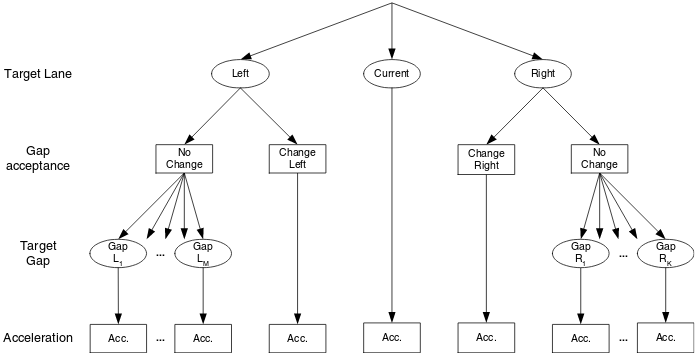
\includegraphics{toledo-2007-behavior-model-tree}
	\caption{Estructura del modelo de comportamiento de los vehículos en \cite{Toledo2007}. El agente comprueba constantemente se desea o no cambiar de carril, y una vez decidido comprueba la viabilidad. En cualquier caso, toda decisión finaliza con la comprobación de la aceleración. Fuente: \cite{Toledo2007}.\TODO{Quizá la imagen es muy grande y quedaría mejor si la hiciésemos más pequeña.}}
	\label{fig:toledo-2007-behavior-model-tree}
\end{figure}

Sin embargo, a partir de los años $90$ se ha tendido al desarrollo de modelos de comportamiento que combinan los modelos de aceleración y de cambio de carril (\cite{Ma2004}). Un ejemplo actual de este tipo de modelos es el descrito en \cite{Toledo2007}, el cual se basa en el concepto de \enquote{objetivo a corto plazo} para elaborar un \enquote{plan a corto plazo} apoyándose en un árbol de decisión que determina la accinó a realizar (ver figura~\ref{fig:toledo-2007-behavior-model-tree}).

...

\section{La \glsentrylong{ci} en los modelos de conducción}

La mayoría de los modelos de comportamiento existentes basan su funcionamiento en técnicas pertenecientes al \glsentrylong{hc}; es decir, están basados en fórmulas matemáticas y reglas de la lógica convencional con parámetros que se ajustan a partir de la observación de datos reales. Sin embargo, desde mediados de los años $90$ empezó a crecer el interés por las técnicas de la \gls{ci}.

...

Según~\cite{Aghabayk2015}, los modelos basados en \acrlongsp{ai} funcionan en base a dos técnicas principalmente, las \acrlongplsp{ann} y la \acrlongsp{fl}.

\subsection{Modelos basados en lógica difusa}

Los modelos de car following que se basan en la lógica difusa suelen apoyarse en la convicción de que la información que maneja el conductor a la hora de tomar decisiones proviene de un análisis no demasiado detallado de la situación que le rodea y que, por tanto, su razonamiento parte de conceptos imprecisos y vagos que conducen a respuestas no demasiado bien definidas.

\cite{Kikuchi1992} fueron los primeros en aplicar lógica difusa a modelos de conducción. Usaron el modelo \gls{ghr}\sidenote{
	El modelo \gls{ghr} es el modelo más conocido antes de la introducción del modelo de Gipps. Desarrollado a finales de los años $50$, calcula el valor de la aceleración $a$ en un instante $t$ como:
	
	\begin{equation}
	a(t) = c v^m(t) \frac{\Delta v(t - \tau)}{\Delta x^l(t - \tau)}
	\label{eq:ghr-car-following-model}
	\end{equation}
	
	Siendo $t$ es el instante actual, $a(t)$ la aceleración del vehículo, $\delta v(t)$ y $\delta x(t)$ son la velocidad y distancia relativas al siguiente coche respectivamente, $v$ la velocidad del vehículo y $c$, $m$, $l$ y $\tau$ constantes, siendo ésta última el tiempo de reacción del conductor.
} (\cite{Chandler1958}). Las entradas al modelo eran distancia al coche delantero, diferencia de velocidades, aceleración y deceleración del coche delantero. La aceleración y deceleración se toman como entradas diferentes porque postulaban que el comportamiento antes ambos casos era diferente (aunque creo que esto es equivalente a usar particiones no simétricas de la variable lingüística. Como salida, la aceleración/decelearación del coche actua

Otros trabajos que trabajan con lógica difusa: (Evaluation of the General Motors based car-following models and a proposed fuzzy inference model, Calibrating the membership functions of the fuzzy inference system: instantiated by car-following data, A FUZZY LOGIC MODEL OF FREEWAY DRIVER BEHAVIOR, The Modeling and Simulation of the Car-following Behavior Based on Fuzzy Inference, Fuzzy parameters estimation for car-following modelling, A Fuzzy Logic Approach for Car-Following Modelling, Variable response time lag module for car-following models, Development of a fuzzy logic based microscopic motorway simulation model, Establishment of car following theory based on fuzzy-based sensitivity parameters. Advances in multimedia modelling, Application of fuzzy systems in the car-following behaviour analysis, The validation of a microscopic simulation model: A methodological case study). Ninguno de estos estudios considera diferentes tipologías de vehículos para el car following

Problemas:

\begin{enumerate}
	\item ¿Qué reglas usan los humanos para modelar su comportamiento? Desconocerlas implica modelos no realistas. En (The validation of a microscopic simulation model: A methodological case study) intenta suplir este problema con encuestas a conductores.
	\item Los problemas inherentes de los controladores difusos. ¿Cómo validar las funciones de pertenencia? ¿cómo determinar las reglas difusas?
\end{enumerate}

\subsection{Modelos basados en redes neuronales artificiales}

Las redes neuronales se han aplicado mucho sobre el campo de las ITS en general, y sobre la conducción autónoma y el análisis del comportamiento de los conductores (A review of neural networks applied to transport).

En (Modelling human performance with neural networks) implementaron un controlador basado en redes neuronales para el comportamiento del car following en un microsimulador entrenando dicho modelo previamente con datos extraídos de un conductor en dicho simulador.

En (The  use  of  neural  networks  to  recognise  and
predict traffic congestion) usan redes para determinar el nivel de congestión en la vía.

(Develop a car-following model using data collected by ‘five-wheel
system’) son los primers en usar datos reales de un coche instrumentado usando el método Five-Wheel-System, que está especificado en su paper de aquella manera y que no me entero de nada. A partir de las entradas correspondientes a velocidad relativa, espacio relativo, velocidad y velocidad deseada (para ello, clasifican al conductor de agresivo, normal, conservador) determinan la aceleración/deceleración del vehículo. No lo aplican a ningún simulador, sólo que los valores se ajustan.

(Neural agent car-following models) redes neuronales usando el dataset de (Traffic simulation supporting urban control system development) desarrollan una red neuronal para mantener la distancia con el siguiente vehículo. Este modelo sí se evaluó en el simulador AIMSUN, y los resultados muestran una buena correspondiencia entre los datos y la realidad. No replica sin embargo el comportamiento de frenar hasta parar o de acelerar desde parado.

Problemas:

\begin{enumerate}
	\item Es imposible determinar por qué la red funciona como está funcionando.
	\item Los clásicos de los problemas de redes, el no aprendizaje y la especialización.
\end{enumerate}

\subsection{Otras técnicas}

\subsection{Aproximaciones híbridas}

(Simulation of car-following decision using fuzzy neural network system) y (Toward an integrated car-following and lane-changing model based on neural-fuzzy approach) usan aproximaciones de fuzzy neural networks y neuro-fuzzy respectivamente. No proveen sin embargo de documentación y no se investiga la aplicación de estos modelos a microsimuladores de tráfico.

(Exploring a local linear model tree approach to car-following) usan el modelo de árboles lineales locales (LOLIMOT, (Nonlinear system identification: From classical approaches to neural networks and fuzzy models)) que no deja de ser una aproximación neuro-fuzzy del comportamiento. Intenta incorporar imperfecciones perceptuales en un modelo de car following. El modelo está basado usando datasets reales y los resultados indican que se ajusta lo predicho con la realidad, pero no hay pruebas realizadas en microsimuladores.

En~\cite{Ma2004}, bajo la suposición de que el ser humano toma múltiples decisiones relacionadas basándose en su percepción (imprecisa) del entorno propone un método masado en un sistema de inferencia difusa para tomar decisiones tanto para el problema del \textit{car following} como para el del \textit{lane changing}, calibrando y ajustando dicho controlador mediante el uso de redes neuronales (aproximación Neuro-Fuzzy).

\section{Por procesar}

SUMO usa (al menos así lo indican en el paper del 2002) el modelo Gipps\cite{krajzewicz2002sumo}. No sé si ellos han hecho una extensión del modelo o están referenciando la extensión y ellos sólo la implementan. En el paper del 2012 citan que el modelo car-following que usan por defecto es el desarrollado por Stefan Krauß\cite{jin2016evaluation}, debido a su simplicidad y su velocidad de ejecución. El modelo ha probado ser válido, pero tiene algunos defectos, por lo que existe un API para implementar otros modelos. En la actualidad están incluidos en el sistema los modelos IDM\cite{treiber2000congested} (\textit{Intelligent Driver Model}), el modelo de tres fases de Kerner\cite{kerner2008testbed} y el modelo de Wiedemann\cite{wiedemann1974simulation}.

En~\cite{sekizawa2007modeling} describen modelos supervisados offline para capturar el comportamiento del conductor basados en auto-regresión a trozos. Más adelante lo extienden en~\cite{terada2010multi}, aunque los datos de entrenamiento son extraídos directamente de simulaciones, no del \enquote{mundo real\textsuperscript{TM}}.

En~\cite{bando2013unsupervised} describen otro modelo no supervisado offline basado en un modelo bayesiano no paramétrico para la clusterización, combinado con un LDA (Latent Dirichlet Allocation, sea lo que sea esto) para la clusterización a más alto nivel. (\TODO ¿este método usa datos reales?)

Estos trabajos (\cite{sekizawa2007modeling}, \cite{terada2010multi} y \cite{bando2013unsupervised}) tienen la desventaja de ser computacionalmente muy costosos y con poca precisión en el caso de variar mucho los escenarios de entrenamiento y de test.

En~\cite{maye2011bayesian} se presenta un modelo online donde se infiere el comportamiento del conductor haciendo uso de una IMU (Intertial Measurement Unit) y una cámara. Primero de la IMU se sacan datos que se separan en fragmentos para luego relacionarlos con las imágenes obtenidas de la cámara. (\TODO ¿Hacia dónde mira la cámara?). Los modelos propuestos en~\cite{johnson2011driving} y~\cite{van2013driver} también se apoyan en el funcionamiento de clasificar las segmentaciones de una IMU, pero con técnicas distintas y sin cámara. Además hacen uso de señales externas y umbrales de activación para hacer más efectiva la clasificación (\TODO corroborar).

En el artículo~\cite{bender2015unsupervised} se usa también un modelo no supervisado online con una aproximación bayesiana para identificar los puntos de cambio sin depender de parámetros externos (e.g. umbrales o señales). Se basa también en (1) segmentar los datos de conducción y (2) asignar estos datos a clases que se corresponde n con comportamientos de conducción. Tiene la ventaja de ser más eficiente y rubusto que los anteriores.

La idea de estos métodos desde el~\cite{sekizawa2007modeling} hasta el~\cite{bender2015unsupervised} creo que es el de un sistema que traduzca datos en crudo a datos de más alto nivel. Esto es debido a que la cantidad de datos que se pueden generar en un sólo coche (no digamos ya una flota de ellos) es tan grande que para determinados sistemas disponer de información de más alto nivel haría más sencillo su desempeño (por ejemplo, \gls{adas} que funcionasen con datos de \enquote{adelantando} que sus valores de giro, aceleración en una ventana temporal).

En~\cite{satzoda2013towards}, haciendo uso de la información combinada de bus CAN, cámaras, GPS e información digitalizada el mapa donde se circula se determina una amplio abanico de información crítica en diferentes condiciones de la carretera. La información que sacan es: número de cambios de carril a la derecha, a la izquierda, tiempo en autopista y carretera urbana, distancia recorrida, velocidades medias en autopista y urbano, paradas, giros a la derecha, a la izquierda, incormporaciones y salidas de autopsta, tiempo gastado en un sólo carril, curvas a la izquierda, curvas a la derecha y distancia media al carril central

En~\cite{al2001framework} describen un framework para la modelización de comportamiento de conductores dentro de simuladores. Se basa en cuatro unidades de funcionamiento interconectadas, la de percepción (percibe el entorno en términos locales y globales), la de emoción (cómo responde emocionalmete al entorno), la de decision-making (investiga posibles acciones que podrían servir a las necesidades del módulo emocional) y la de decision-implementation (intenta implementar las decisiones cuando emergen condiciones de tráfico lo suficientemente seguras para llevarlas a cabo). Tengo que volver a leerlo después de hacer una primera introducción en el tema de agentes, porque me parece poner nombrecitos a un tipo de agente que funciona de esa misma manera, pero lo mismo no.

En~\cite{terroso2015complex} analizan lo que ellos denominan el concepto del \gls{ivca}, lo que viene a ser el contexto definido \textbf{dentro} del vehículo, llegando a intentar predecir no sólo el número de ocupantes (ese es un problema sobradamente superado) sino la tipología o clase de ocupante (e.g. niños, adultos, ... \TODO buscar cuáles son las tipologías). Para ello hacen uso de un \gls{cep}\footnote{Un \gls{cep} es un método por el cual se lee un flujo de información compuesta de flujos de distintas fuentes (de ahí el \textit{complex}) para detectar eventos o patrones que pueden indicar la presencia de situaciones a analizar lo más rápido posible.} para procesar los datos de los diferentes sensores del vehículo y así detectar y analizar patrones característicos.

El artículo~\cite{munoz2010human} es muy interesante ya que para la competición \textit{2010 Simulated Car Racing Championship} desarrollaron un controlador no para minimizar el tiempo en realizar las carreras, sino para hacerlo lo más parecido posible a cómo se comporta un humano. Para ello hicieron uso de redes neuronales para calcular trayectorias y de un proceso de aprendizaje a partir de información extraída de un conductor real en el simulador \gls{torcs}.

Aunque \gls{torcs} es usado como entorno de simulación en diversos concursos e investigaciones, se trata de un juego, y es que los juegos son un sandbox perfecto como entorno de simulación, ya que presentan una abstracción del dominio sobre el que trabajar. Otros trabajos en esta línea (entrenamiento de redes neuronales en este simulador) son los de~\cite{munoz2009controller} y~\cite{van2009robust}, el primero entrenando perceptrones multicapa (\TODO verificar) con un backpropagation haciendo uso de un dataset proporcionado por un bot y otro haciendo uso de un algoritmo evolutivo multiobjetivo para optimizar la red de acuerdo a un conjunto de datos proporcionado por un conductor real. Sin embargo, este tipo de modelos se encuentran más cercanos al nivel de control que al nivel de maniobra descritos en la figura~\ref{fig:three-levels-of-human-driving}.

En~\cite{van2013driver} hacen uso de los sensores de inercia de un coche (a saber qué coche tienen) para construir un perfil de conductor. Concluyen que frenar y girar caracterizan mejor a los conductores frente a acelerar.

En \cite{Das} se realiza una simulación de comportamiento de vehículos en autopista. Los agentes basan su comoprtamiento en un sistema difuso donde las reglas definen la cnclusión en autopista (i.e. car-following y lane-changing). Llaman a este simulador AASIM (Autonomous Agent Simulator).,

En \cite{Dia2002} Los parámetros relativos al comportamiento, es decir, los que definen características, forma de razonar, etcétera son extraídos deencustas a conductores reales. De acuerdo a los autores, cada conductor cno sus propias características su forma de razonar sus perceciones y sus objetivos se puede modelar como un agente.

En \cite{Ehlert2001} (ver si este otro paper del autor cuenta lo mismo y me quito de una de las dos referencias: \cite{Ehlert2001-2}), simulación donde los agentes son de tipo reactivo. Además, poseen diferentes estuilos de conduccińo. El agente cntinuamente va realizando decisiones de control para mantenerse en la via y llegar a su destino.

En \cite{} definen dos capas, \enquote{física} y \enquote{mental}. La física es aquella donde los agentes se mueven de acuerdo a sus magnitudes físicas, evitando accidentes y, en resumen, comportándose al volante. La mental es la que se encarga de las estrategias a más alto nivel, como por ejemplo la actividad planeada o la ruta escogida. Los parámetros de los agentes y de la simulación son extraídos de censos y encuestas.